\section{CMOS MAPS}

    %%%%%%%%%%%%%%%%%%%%%%%%%%%%%%%%%%%%%%%%
    %%  Slide 2: <CMOS MAPS concept>  %%
    %%%%%%%%%%%%%%%%%%%%%%%%%%%%%%%%%%%%%%%%
    \begin{frame}
        \frametitle{CMOS MAPS: signal formation}
        %forse anche la terza parentesi con minore circa 100 um
        %Few sensor types depending on the electrode shape
        \begin{columns}
            \column{0.6\textwidth}
                \vspace*{-0.5cm}
                \hspace*{+1.2cm}
                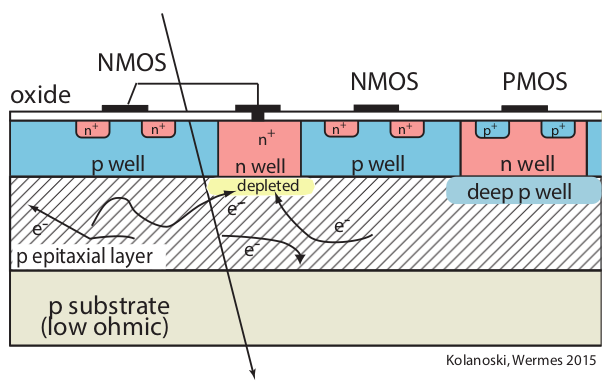
\includegraphics[width=0.9\linewidth]{figures/Pixel_detectors/MAPS_scheme.png}
                \column{0.1\textwidth}  
                \column{0.2\textwidth}  
                \begin{tikzpicture}[overlay]
                    \draw[decorate,decoration={brace}]
                        (-1.6, +1.2) -- node[xshift=2pt,anchor=west] {$\lesssim$\SI{5}{\um} electronics}(-1.6, 0.5);
                \medskip
                    \draw[decorate,decoration={brace}]
                        (-1.6, 0.4) -- node[xshift=2pt,anchor=west] {$\lesssim$\SI{50}{\um} sensor}(-1.6,-0.5);
                \end{tikzpicture}
            \end{columns}   
        \medskip \bigskip
            Signal produced by a particle:\\
            \medskip
            \begin{itemize}
                %\item An epitaxial layer with doping few order of magnitude smaller than the subtrate is introduced below the surface
                \item e/h created by ionization $\rightarrow$ in Si @ \SI{300}{K}, $w_{i}$=\SI{3.6}{eV}
                \item by the motion of charge, by drift or diffusion  
            \end{itemize}
            \bigskip
            \begin{equation*}%\hspace{-100pt}\vspace{-65pt}
                Q_{MIP}\propto d \sim 80 e^-/\si{\um}
            \end{equation*} 


    \end{frame} 

    %%%%%%%%%%%%%%%%%%%%%%%%%%%%%%%%%%%%%%%%
    %%  Slide 2: <CMOS MAPS concept>  %%
    %%%%%%%%%%%%%%%%%%%%%%%%%%%%%%%%%%%%%%%%
    \begin{frame}
        \frametitle{CMOS Monolithic Active Pixel Sensors}
        %forse anche la terza parentesi con minore circa 100 um
        \begin{columns}
            \column{0.6\textwidth}
                \vspace*{-0.5cm}
                \hspace*{+1.2cm}
                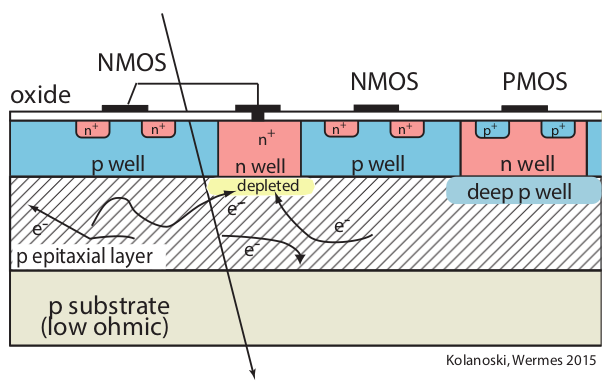
\includegraphics[width=0.9\linewidth]{figures/Pixel_detectors/MAPS_scheme.png}
                \column{0.1\textwidth}  
                \column{0.2\textwidth}  
                \begin{tikzpicture}[overlay]
                    \draw[decorate,decoration={brace}]
                        (-1.6, +1.2) -- node[xshift=2pt,anchor=west] {$\lesssim$\SI{5}{\um} electronics}(-1.6, 0.5);
                \medskip
                    \draw[decorate,decoration={brace}]
                        (-1.6, 0.4) -- node[xshift=2pt,anchor=west] {$\lesssim$\SI{50}{\um} sensor}(-1.6,-0.5);
                \end{tikzpicture}
            \end{columns}   
        \medskip         
        \begin{itemize}
            \item High resistivity $\rho$ allows for fully depleted epi-layer Depleted-MAPS at sufficiently low bias $V$: 
             $d \propto \sqrt{\rho V}$
            \item $V = Q/C$ $\rightarrow$ if the sensor capacitance C is sufficiently low:
            \begin{itemize}
                \item High signal and good \textbf{S/N} performances  
                \item High \textbf{gain} for the first amplification stage
            \end{itemize}
        \end{itemize}
                %\begin{equation*}
                %    \hspace{40pt} d \propto \sqrt{\rho V}
                %\end{equation*}              
                %\begin{equation*}
                %    \hspace{40pt} V = \frac{Q}{C}
                %\end{equation*} 
                %\begin{equation*}
                %    \hspace{80pt} ENC^2 \propto C_D ^2
                %\end{equation*}  
                %\begin{equation*}
                %    \hspace{80pt} \tau \propto C_D
                %\end{equation*}  
    \end{frame} 

    %%%%%%%%%%%%%%%%%%%%%%%%%%%%%%%%%%%%%%%%
    %%  Slide 1: <READOUT>  %%
    %%%%%%%%%%%%%%%%%%%%%%%%%%%%%%%%%%%%%%%%
    \begin{frame}
        \frametitle{Front end electronics}
            \begin{columns}
                \column{0.7\textwidth}  
                Pitch$\sim$\SI{50}{\um} $\rightarrow$ \textbf{pixel area economy} and dimension of components are extremely relevant. \\\smallskip
                MAPS usage allowed by miniaturization of components, i.e. TJ-Monopix1 is 180{nm} CMOS process.\\
                \column{0.4\textwidth}  
                    \begin{figure}[h!]
                        \vspace*{-0.9cm}\hspace*{-0.9cm}
                        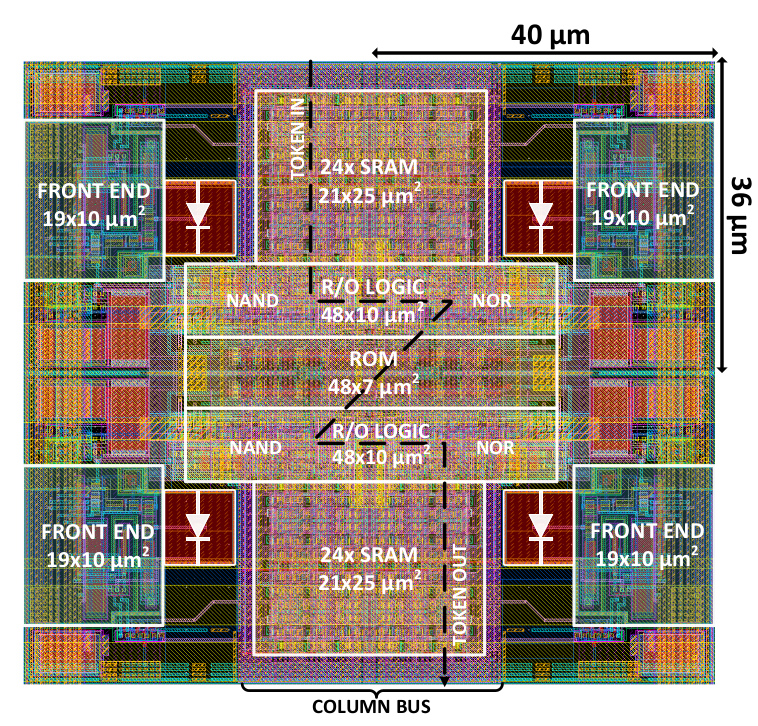
\includegraphics[width=1.1\linewidth]{figures/Monopix1/Monopix1_2x2pixelsgroup.png}
                    \end{figure}
            \end{columns}

            \begin{columns}
                \column{0.45\textwidth} 
                    The pixel area include the:
                    \begin{itemize}
                        \item Electrode
                        \item Analog front end
                        \item Digital readout 
                    \end{itemize} 
                \column{0.55\textwidth} 
                    \vspace*{-0.15cm}%\hspace*{+0.15}
                    \begin{beamercolorbox}[rounded=true, center]{palette light primary}
                        \setlength{\tabcolsep}{0.5em} % for the horizontal padding
                        {\renewcommand{\arraystretch}{1.2}% for the vertical padding
                        \begin{tabular}{l|l}
                            Analog & Digital\\
                            \hline
                            Triggered & Triggerless\\
                            \hline
                            Buffer & No buffer \\
                            \hline
                            Rolling shutter & Sparsified\\
                        \end{tabular}
                        }
                    \end{beamercolorbox}
            \end{columns}
    \end{frame} 


